\documentclass[letterpaper,journal]{IEEEtran}
\usepackage{amsmath,amssymb}
\usepackage{graphicx}
\usepackage{booktabs}
\usepackage{array}
\usepackage{xcolor}
\usepackage{url}
\usepackage{cite}
\usepackage{tikz}
\usetikzlibrary{positioning,arrows.meta,fit,calc}
\usepackage[hidelinks]{hyperref}

\newcommand{\dnet}{\mathbf{d}_{\mathrm{net}}}
\newcommand{\dgeo}{\mathbf{d}_{\mathrm{geo}}}

\begin{document}

\title{Measure What Is Observable, Learn the Rest:\\Observability-Gated Fusion for Learned Visual--Inertial Odometry}

\author{Nada El Madah%
\thanks{Manuscript in preparation. Code and Kaggle kernels: to be released.}}

\markboth{Preprint, 2026}{Measure What Is Observable, Learn the Rest}

\maketitle

\begin{abstract}
Satellite positioning stops at the door. Inside a warehouse, a hospital or a mine, an indoor positioning system (IPS) must tell a robot, drone or headset where it is, and a natural way is to track its motion with only a camera and an inertial sensor (IMU), the pair found in every phone: visual--inertial odometry (VIO). A gyroscope measures rotation. An accelerometer can measure step length. Two views of a scene give the direction of travel. Yet learned VIO asks one neural network to predict all of it, and this is where it fails. Swapping one pose component at a time for ground truth shows where: for a recent transformer VIO model, rotation and step length on KITTI and translation direction on EuRoC. The swap also exposes a 4\% timing error in the KITTI inertial files distributed with several released models (their 100\,Hz samples span a $\approx$104\,ms image interval, not 100\,ms) that had made the gyroscope look worse than the network. We propose an \emph{observability gate} that, for every frame pair and pose component, uses the sensor measurement where the sensors observe that component and the frozen network elsewhere, deciding from sensor signals alone (parallax, solver uncertainty, conditioning, gravity consistency). With one configuration, fixed on held-out data and pre-registered, the gate reduces KITTI translation error from the 1.96\% published for that model to 1.56\% without test-set model selection (1.65\% against IMU-independent lidar poses), lowers EuRoC error from 5.5--6.6\,m to below 1\,m, and cuts the error of three released models we did not train by 45--59\%. It is not flawless: on TUM-VI it over-trusts the network, and a post-hoc revision that estimates this trust online removes the failure. The rule: measure what is observable, learn the rest, and measure how far to trust what you learn.
\end{abstract}

\begin{IEEEkeywords}
Visual--inertial SLAM, deep learning methods, sensor fusion, localization.
\end{IEEEkeywords}

\section{Introduction}

\IEEEPARstart{T}{o} move through the world without satellite positioning, a robot, drone or headset must track its own motion. Visual--inertial odometry (VIO) does this with a camera and an inertial sensor (IMU): for each pair of consecutive frames it estimates how the camera rotated, and in which direction and how far it moved.

Learned VIO trains one neural network to predict all of this at once, from recurrent models \cite{Clark2017,Han2019} to visual modality selection \cite{Yang2022} and transformers over frozen visual and inertial latents \cite{Kurt2024}. Published models report a relative translation error $t_\mathrm{rel}$ of 1.69--1.96\% on KITTI \cite{Kurt2024,Ma2026,Wan2026}; these gains come from inside the network: rotation losses \cite{Chen2022}, longer context, new fusion modules.

The sensors, however, already measure much of the pose: a gyroscope measures rotation, an accelerometer can measure the step length, and two-view geometry measures the direction of travel once rotation is known. So we ask \emph{which part of the pose is wrong}, rather than how to improve the whole network. An oracle swap answers this without retraining: replace one predicted component by ground truth and re-score. On KITTI, for the transformer model VIFT \cite{Kurt2024} (released-code split), ground-truth rotation with the network's own translation already scores 1.55\%, better than the 1.96\% VIFT reports: rotation is the main problem.

Yet integrating the gyroscope windows that the network receives gives 4.62\%, far worse than the network. The reason is a timing detail: the inertial windows distributed with several released models \cite{Yang2022,Kurt2024,Chen2023NASVIO,Park2024ULVIO} hold 11 samples per image pair, which suggests 10\,ms steps, but they are the raw 100\,Hz readings interpolated over the \emph{actual} image interval, which is $\approx$104\,ms on KITTI. Integrating with the nominal step under-rotates every frame by 4\% and makes an accurate gyroscope look biased; over the true interval it gives 1.70\% with $r_\mathrm{rel}$ 0.18. The networks themselves never see the step, so only methods that integrate these files inherit the error. For drive 05 the file is byte-identical (MD5) across these four. Newer models that integrate the gyroscope explicitly, such as DB-VIO \cite{Wan2026}, also use 11 interpolated samples per pair but do not state their time step; we have not checked whether they are affected.

On EuRoC the same swap points at a different component, the translation direction, which the camera measures geometrically once rotation is known; on TUM-VI the network direction is 40--87$^\circ$ off.

This suggests a design rule: measure each component where the sensors observe it, and learn only the rest. Observability varies along a trajectory (the step length is unobservable at a stop or at constant velocity, the direction at tiny parallax), so the choice must be made per edge.

\textbf{Contributions.}
\begin{enumerate}
\item A component-wise oracle-swap diagnosis of learned VIO, including the KITTI $\approx$104\,ms / +60\,ms timing finding, showing that the failing component is dataset-dependent.
\item An observability gate that chooses between sensor measurements and a frozen network per edge and per component from sensor-computable signals only, pre-registered on KITTI, EuRoC and TUM-VI and run frozen on three released models we did not train, with every failure reported; and a post-hoc online estimate of the network's trustworthiness that removes the TUM-VI failure.
\item Measurement components validated against references independent of the IMU (lidar SLAM, motion capture), a protocol audit of VIFT, and an analysis of what remains.
\end{enumerate}

\section{Related Work}

\textbf{Classical VIO.} Filtering \cite{Mourikis2007} and optimization \cite{Leutenegger2015,Qin2018,Campos2021} integrate the gyroscope between frames with accurate timestamps and calibrated camera--IMU offsets \cite{Furgale2013,Qin2018b}. With rotation known, relative pose reduces to a two-point problem \cite{Kneip2011,Troiani2014}, and metric scale and gravity follow from a linear visual--inertial alignment \cite{Martinelli2014,Qin2017}. We reuse these ingredients inside a learned pipeline.

\textbf{Learned VIO.} VINet \cite{Clark2017}, DeepVIO \cite{Han2019}, SelfVIO \cite{Almalioglu2022}, VS-VIO \cite{Yang2022} and VIFT \cite{Kurt2024} learn the full pose; DB-VIO \cite{Wan2026} injects a gyro-integrated attitude prior into a dual-branch network, MixVIO \cite{Ma2026} selects modalities with phase-aware attention, Diff-VIO \cite{Qin2026} refines learned poses with a diffusion model, and DAP-Pose \cite{DAPPose} aligns modalities in time and adds GNSS. All of them learn components that a sensor measures; we instead decide, per edge, which components to learn at all. Learned inertial odometry \cite{Liu2020,Herath2020} and AI-IMU \cite{Brossard2020} address the inertial side only.

\textbf{Component analysis.} RAUM-VO \cite{Cimarelli2022} substitutes ground-truth rotation and translation into an unsupervised monocular VO network and replaces the learned rotation by an epipolar one at inference. We extend the substitution to learned VIO, to a third component (step length) and to datasets where the failing component is the translation direction. A GNSS-aided pipeline also takes orientation from the gyroscope and translation from learned flow inside a filter \cite{Kang2025}.

\section{Diagnosis}
\label{sec:diag}

\textbf{Oracle swap.} Given per-edge relative poses $(\hat{\mathbf{R}}_k,\hat{\mathbf{t}}_k)$ and ground truth $(\mathbf{R}_k,\mathbf{t}_k)$, we compose trajectories that take each component (rotation, translation direction, step length) from either source and re-score them. Table~\ref{tab:oracle} summarizes the result.

\begin{table}[t]
\caption{Oracle swaps. KITTI: our VIFT reproduction (released code, with-08 split, checkpoint selected on the test drives as in VIFT's code), $t_\mathrm{rel}$\,\% / $r_\mathrm{rel}$\,$^\circ$/100\,m, mean of 05/07/10. EuRoC: learned models, SE(3) ATE (m), MH\_05/V2\_02/V1\_01/V1\_02.}
\label{tab:oracle}
\centering\small
\setlength{\tabcolsep}{4pt}
\resizebox{\columnwidth}{!}{\begin{tabular}{@{}llc@{}}
\toprule
& Rotation / translation & Result \\
\midrule
KITTI & network / network & 2.11 / 0.67 \\
& GT / network & \textbf{1.55} / 0.00 \\
& gyro, nominal 10\,ms steps / network & 4.62 / 1.54 \\
& gyro, true steps / network & \textbf{1.70} / 0.18 \\
& gyro, true steps / GT & 0.39 / 0.18 \\
& VIFT \cite{Kurt2024} & 1.96 / 0.46 \\
\midrule
EuRoC & zero-motion floor & 3.15 \\
& network / network & 4.02--4.98 \\
& GT / network & $\geq$ floor (exc.\ MH\_05) \\
& network / GT & 0.6--2.1 (one run 4.5) \\
& network direction error (median) & 31--90$^\circ$ \\
\bottomrule
\end{tabular}}
\end{table}

\textbf{KITTI: rotation, then length.} With ground-truth rotation the network translation scores 1.55\%. The network's per-frame rotation noise is small (0.014--0.034$^\circ$); the damage is a bias of a few thousandths of a degree per frame; its yaw component changes sign between drives, and constant corrections gain at most 0.13 points, none beating VIFT. A gyroscope should remove it, yet integrating VIFT's inertial windows with the nominal 10\,ms step gives 4.62\%.

\textbf{The timing finding.} We recovered the raw 100\,Hz OXTS stream and image timestamps from the public KITTI raw archives. VIFT's inertial windows equal the raw stream linearly interpolated at ten equal sub-steps of the \emph{true} image interval, which is 103.7--104.1\,ms on drives 04--10. Integrating over the true interval (trapezoidal rule on raw sample times) gives a median per-frame error of 0.023--0.037$^\circ$ and 1.70\% / 0.18 with the network translation. The integration window of each edge is shifted by a constant lag between the image timestamps and the odometry ground truth, and rotated by the IMU-to-camera rotation; both are fitted on training drives only (Fig.~\ref{fig:timing}). The lag is $+60$\,ms ($+62.5$\,ms on one recording day), and its physical origin is unresolved. KITTI's cameras are triggered by the lidar spin \cite{Geiger2013}; learned-VIO work assumes a nominal 10\,Hz \cite{Yang2022,Kurt2024,Wan2026,Almalioglu2022}, and we found no prior measurement of the 104\,ms period or the 60\,ms offset. With the gyro rotation and the network translation fixed, the next component the swap points at is the step length.

\textbf{EuRoC: direction.} Here ground-truth rotation gives no gain, while ground-truth translation drops ATE below the zero-motion floor on three of four sequences. The learned direction error grows with distance from the training rooms (PI-VIFT: 53$^\circ$ on MH\_05, four training sequences in the same room; 66$^\circ$ on V2\_02, one; 70--90$^\circ$ on V1, none), approaching a random direction. Neither an up-to-scale direction loss \cite{Wang2020} nor unfreezing the encoder made it transfer (one seed each; ATE 6.60 and 3.60\,m). On TUM-VI, where we did not run the swap, the network direction is 40--87$^\circ$ off and its length 14--83\% too long.

\begin{figure}[t]
\centering
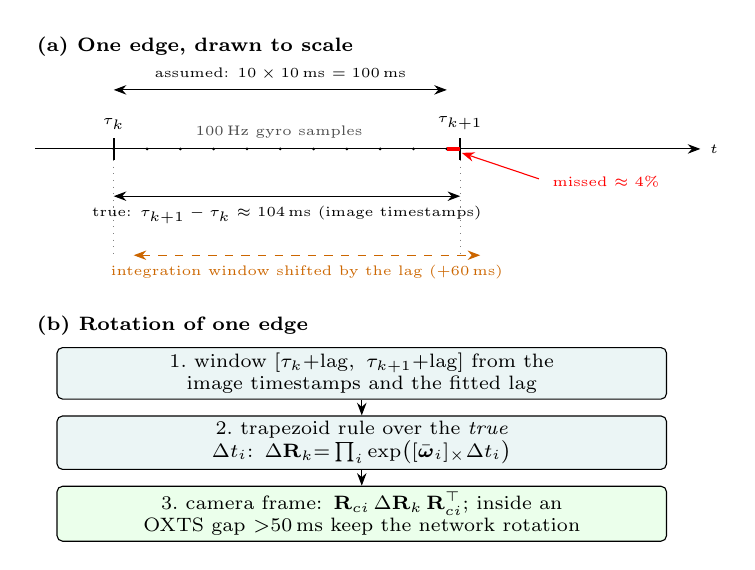
\begin{tikzpicture}[font=\scriptsize, >={Stealth[length=1.6mm]},
  st/.style={draw, rounded corners=2pt, align=center, inner sep=2pt, text width=7.6cm, minimum height=5.2mm, fill=teal!8},
  ttl/.style={font=\scriptsize\bfseries, anchor=west}]
% (a) one edge, to scale (1 ms = 0.0423 cm)
\node[ttl] at (-0.1,1.3) {(a) One edge, drawn to scale};
\draw[->] (0,0) -- (8.45,0) node[right, font=\tiny] {$t$};
\foreach \j in {0,...,10} {\fill ({1.0+0.423*\j},0) circle (0.55pt);}
\node[font=\tiny, gray!60!black] at (3.1,0.22) {100\,Hz gyro samples};
\draw[thick] (1.0,-0.14) -- (1.0,0.14); \node[above, font=\tiny] at (1.0,0.12) {$\tau_k$};
\draw[thick] (5.4,-0.14) -- (5.4,0.14); \node[above, font=\tiny] at (5.4,0.12) {$\tau_{k+1}$};
\draw[red, very thick] (5.23,0) -- (5.4,0);
\draw[<->] (1.0,0.75) -- (5.23,0.75) node[midway, above, font=\tiny] {assumed: $10\times10$\,ms $=100$\,ms};
\node[red, font=\tiny, anchor=west] at (6.45,-0.42) {missed $\approx4\%$};
\draw[red, ->] (6.4,-0.38) -- (5.42,-0.05);
\draw[<->] (1.0,-0.6) -- (5.4,-0.6) node[midway, below, font=\tiny] {true: $\tau_{k+1}-\tau_k\approx104$\,ms (image timestamps)};
\draw[dotted, gray] (1.0,-0.14) -- (1.0,-1.35); \draw[dotted, gray] (5.4,-0.14) -- (5.4,-1.35);
\draw[<->, dashed, orange!80!black] (1.254,-1.35) -- (5.654,-1.35) node[midway, below, font=\tiny] {integration window shifted by the lag ($+60$\,ms)};
% (b) steps
\node[ttl] at (-0.1,-2.25) {(b) Rotation of one edge};
\node[st] (s1) at (4.15,-2.85) {1.\ window $[\tau_k{+}\mathrm{lag},\ \tau_{k+1}{+}\mathrm{lag}]$ from the image timestamps and the fitted lag};
\node[st, below=2mm of s1] (s2) {2.\ trapezoid rule over the \emph{true} $\Delta t_i$: $\Delta\mathbf{R}_k{=}\prod_i \exp\!\big([\bar{\boldsymbol\omega}_i]_\times \Delta t_i\big)$};
\node[st, below=2mm of s2, fill=green!8] (s3) {3.\ camera frame: $\mathbf{R}_{ci}\,\Delta\mathbf{R}_k\,\mathbf{R}_{ci}^{\top}$; inside an OXTS gap ${>}50$\,ms keep the network rotation};
\draw[->] (s1) -- (s2); \draw[->] (s2) -- (s3);
\end{tikzpicture}
\caption{Gyro rotation over the true image interval. (a) VIFT's inertial windows hold 11 samples per image pair, read as ten 10\,ms steps, but the image interval is $\approx$104\,ms, so every edge loses $\approx$4\% of its rotation. (b) Pipeline. The lag and the IMU-to-camera rotation $\mathbf{R}_{ci}$ are fitted on training drives only: the lag on a grid from $-80$ to $+80$\,ms (10\,ms, then 2.5\,ms steps) minimizing the median residual after a Kabsch alignment.}
\label{fig:timing}
\end{figure}

\section{Method}
\label{sec:method}

\begin{figure*}[t]
\centering
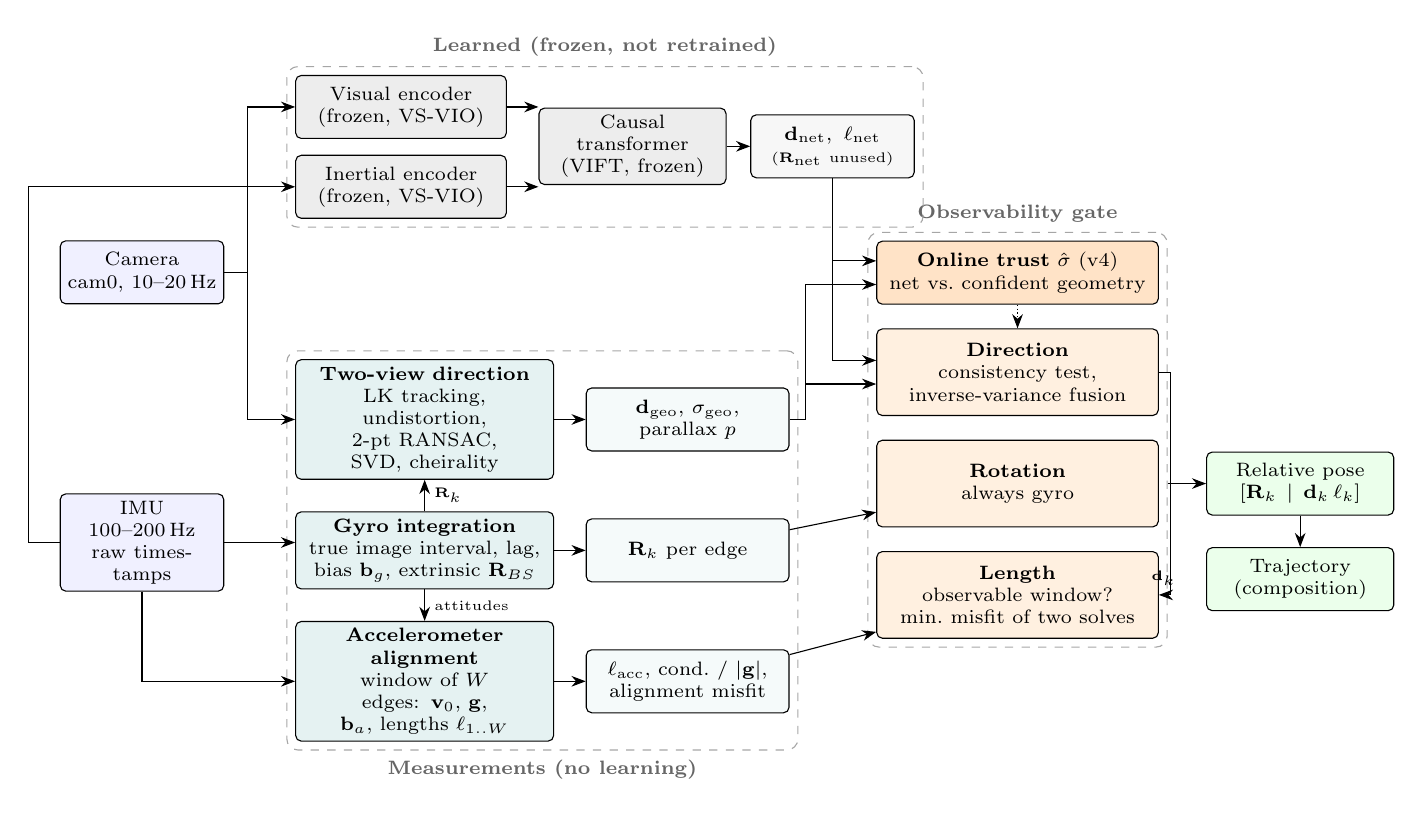
\begin{tikzpicture}[font=\scriptsize, >={Stealth[length=1.8mm]}, node distance=3mm,
  blk/.style={draw, rounded corners=2pt, align=center, inner sep=2.5pt, minimum height=8mm, text width=#1},
  blk/.default=25mm,
  inp/.style={blk=19mm, fill=blue!6},
  lrn/.style={blk, fill=gray!14},
  mea/.style={blk=31mm, fill=teal!10},
  gat/.style={blk=34mm, fill=orange!12, minimum height=11mm},
  res/.style={blk=22mm, fill=green!8},
  lane/.style={draw, dashed, rounded corners=4pt, inner sep=3pt, gray!70},
  lab/.style={font=\scriptsize\bfseries, gray!80!black}]
% inputs
\node[inp] (cam) {Camera\\cam0, 10--20\,Hz};
\node[inp, below=24mm of cam] (imu) {IMU\\100--200\,Hz\\raw timestamps};
% learned lane
\node[lrn, right=9mm of cam, yshift=21mm] (venc) {Visual encoder\\(frozen, VS-VIO)};
\node[lrn, below=2mm of venc] (ienc) {Inertial encoder\\(frozen, VS-VIO)};
\node[lrn, right=4mm of venc, yshift=-5mm, text width=22mm] (tr) {Causal transformer\\(VIFT, frozen)};
\node[blk=19mm, right=3mm of tr, fill=gray!6] (nout) {$\dnet,\ \ell_{\mathrm{net}}$\\{\tiny($\mathbf{R}_{\mathrm{net}}$ unused)}};
% measurement lane
\node[mea, right=9mm of imu, yshift=-1mm] (gyr) {\textbf{Gyro integration}\\true image interval, lag,\\bias $\mathbf{b}_g$, extrinsic $\mathbf{R}_{BS}$};
\node[mea, above=4mm of gyr] (geo) {\textbf{Two-view direction}\\LK tracking, undistortion,\\2-pt RANSAC, SVD, cheirality};
\node[mea, below=4mm of gyr] (acc) {\textbf{Accelerometer alignment}\\window of $W$ edges: $\mathbf{v}_0$, $\mathbf{g}$,\\$\mathbf{b}_a$, lengths $\ell_{1..W}$};
\node[blk=24mm, right=4mm of geo, fill=teal!4] (geoo) {$\dgeo$, $\sigma_{\mathrm{geo}}$,\\parallax $p$};
\node[blk=24mm, right=4mm of gyr, fill=teal!4] (gyro) {$\mathbf{R}_k$ per edge};
\node[blk=24mm, right=4mm of acc, fill=teal!4] (acco) {$\ell_{\mathrm{acc}}$, cond.\ / $|\mathbf{g}|$,\\alignment misfit};
% gate
\node[gat, right=11mm of geoo, yshift=6mm] (gd) {\textbf{Direction}\\consistency test,\\inverse-variance fusion};
\node[gat, below=3mm of gd] (gr) {\textbf{Rotation}\\always gyro};
\node[gat, below=3mm of gr] (gl) {\textbf{Length}\\observable window?\\min.\ misfit of two solves};
\node[gat, above=3mm of gd, minimum height=8mm, fill=orange!22] (trust) {\textbf{Online trust} $\hat\sigma$ (v4)\\net vs.\ confident geometry};
\node[lane, fit=(trust)(gd)(gr)(gl), label={[lab]above:Observability gate}] (gate) {};
% output
\node[res, right=6mm of gr] (pose) {Relative pose\\$[\mathbf{R}_k \mid \mathbf{d}_k\,\ell_k]$};
\node[res, below=4mm of pose] (traj) {Trajectory\\(composition)};
% lanes
\node[lane, fit=(venc)(ienc)(tr)(nout), label={[lab]above:Learned (frozen, not retrained)}] {};
\node[lane, fit=(geo)(gyr)(acc)(geoo)(gyro)(acco), label={[lab]below:Measurements (no learning)}] {};
% arrows
\draw[->] (cam.east) -- ++(3mm,0) |- (venc.west);
\draw[->] (imu.west) -- ++(-4mm,0) |- (ienc.west);
\draw[->] (venc.east) -- (tr.west|-venc.east);
\draw[->] (ienc.east) -- (tr.west|-ienc.east);
\draw[->] (tr) -- (nout);
\draw[->] (cam.east) -- ++(3mm,0) |- (geo.west);
\draw[->] (imu.east) -- (gyr.west|-imu.east);
\draw[->] (imu.south) |- (acc.west);
\draw[->] (gyr) -- node[right, font=\tiny]{$\mathbf{R}_k$} (geo);
\draw[->] (gyr) -- node[right, font=\tiny]{attitudes} (acc);
\draw[->] (geo) -- (geoo); \draw[->] (gyr) -- (gyro); \draw[->] (acc) -- (acco);
\draw[->] (nout.south) |- ([yshift=1.5mm]trust.west);
\draw[->] (nout.south) |- ([yshift=1.5mm]gd.west);
\draw[->] (geoo.east) -- ++(2mm,0) coordinate (gj) |- ([yshift=-1.5mm]gd.west);
\draw[->] (gj) |- ([yshift=-1.5mm]trust.west);
\draw[->] (gyro) -- (gr);
\draw[->] (acco) -- (gl);
\draw[->] (gd.east) -- ++(1.5mm,0) |- node[pos=0.8, above, font=\tiny]{$\mathbf{d}_k$} (gl.east);
\draw[->, densely dotted] (trust) -- (gd);
\draw[->] (gate.east|-gr) -- (pose);
\draw[->] (pose) -- (traj);
\end{tikzpicture}
\caption{System architecture. Camera and IMU feed two branches. The learned branch is a frozen VIFT model (frozen VS-VIO encoders and a causal transformer); only its translation direction $\dnet$ and length $\ell_{\mathrm{net}}$ are used. The measurement branch computes the gyro rotation over the true image interval, the two-view translation direction with that rotation known, and the step length from a windowed accelerometer alignment, each with a quality signal (uncertainty, parallax, conditioning or gravity norm, misfit). The observability gate combines them per edge and per component; the online-trust block (v4) estimates how far the network can be trusted from its agreement with confident geometry.}
\label{fig:pipeline}
\end{figure*}

Fig.~\ref{fig:pipeline} shows the pipeline and Fig.~\ref{fig:net} the learned branch. Each edge $k$ joins two images $\approx$100\,ms apart; its relative pose is $[\mathbf{R}_k \mid \mathbf{d}_k \ell_k]$ with unit direction $\mathbf{d}_k$ and length $\ell_k$.

\begin{figure*}[t]
\centering
\resizebox{\textwidth}{!}{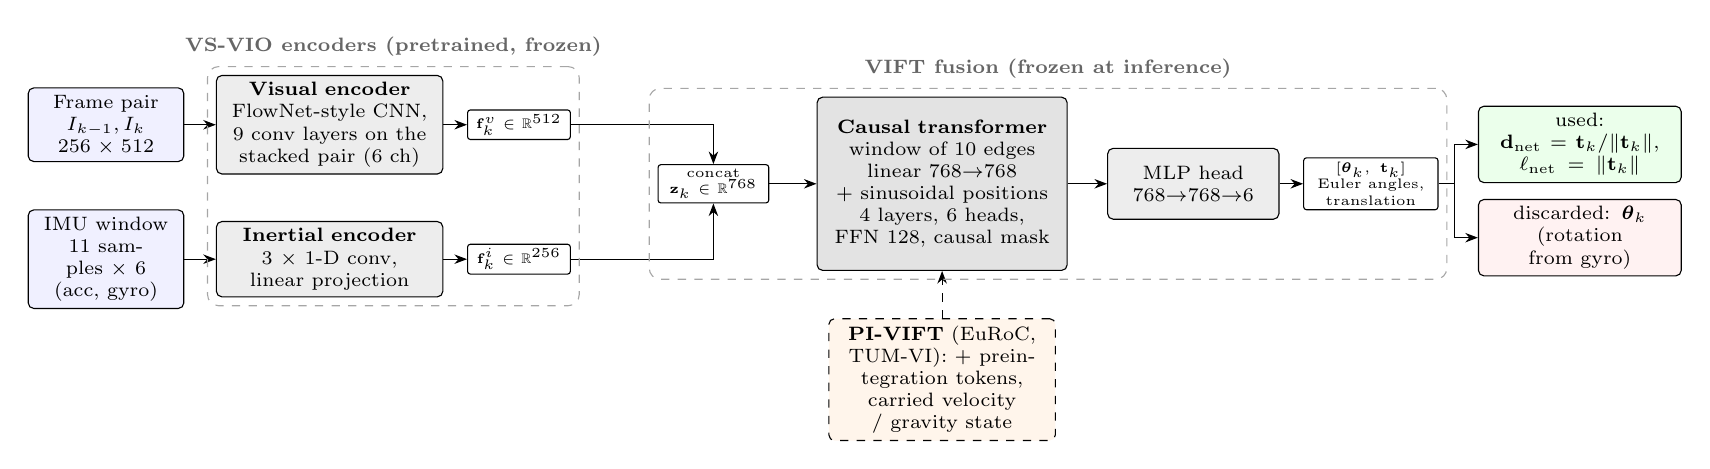
\begin{tikzpicture}[font=\scriptsize, >={Stealth[length=1.6mm]}, node distance=4mm,
  blk/.style={draw, rounded corners=2pt, align=center, inner sep=2.5pt, minimum height=9mm, text width=#1},
  blk/.default=22mm,
  inp/.style={blk=18mm, fill=blue!6},
  enc/.style={blk=27mm, fill=gray!14},
  tf/.style={blk=30mm, fill=gray!22, minimum height=22mm},
  ten/.style={draw, rounded corners=1pt, fill=white, align=center, inner sep=1.5pt, font=\tiny, text width=#1},
  ten/.default=12mm,
  use/.style={blk=24mm, fill=green!8},
  var/.style={blk=27mm, fill=orange!8, dashed},
  lab/.style={font=\scriptsize\bfseries, gray!80!black}]
\node[inp] (imgs) {Frame pair\\$I_{k-1}, I_k$\\$256\times512$};
\node[inp, below=6mm of imgs] (imus) {IMU window\\11 samples $\times$ 6\\(acc, gyro)};
\node[enc, right=of imgs] (venc) {\textbf{Visual encoder}\\FlowNet-style CNN,\\9 conv layers on the\\stacked pair (6 ch)};
\node[enc, right=of imus] (ienc) {\textbf{Inertial encoder}\\3 $\times$ 1-D conv,\\linear projection};
\node[ten, right=3mm of venc] (vf) {$\mathbf{f}^v_k\in\mathbb{R}^{512}$};
\node[ten, right=3mm of ienc] (if) {$\mathbf{f}^i_k\in\mathbb{R}^{256}$};
\node[ten, text width=13mm, right=11mm of vf, yshift=-7.5mm] (z) {concat\\$\mathbf{z}_k\in\mathbb{R}^{768}$};
\node[tf, right=6mm of z] (tf) {\textbf{Causal transformer}\\window of 10 edges\\linear $768{\to}768$\\+ sinusoidal positions\\4 layers, 6 heads,\\FFN 128, causal mask};
\node[blk=20mm, right=5mm of tf, fill=gray!14] (head) {MLP head\\$768{\to}768{\to}6$};
\node[ten, text width=16mm, right=3mm of head] (pose) {$[\boldsymbol{\theta}_k,\ \mathbf{t}_k]$\\Euler angles,\\translation};
\node[use, right=5mm of pose, yshift=5mm] (used) {used: $\dnet=\mathbf{t}_k/\|\mathbf{t}_k\|$,\\$\ell_{\mathrm{net}}=\|\mathbf{t}_k\|$};
\node[blk=24mm, below=2mm of used, fill=red!5] (unused) {discarded: $\boldsymbol{\theta}_k$\\(rotation from gyro)};
\node[var, below=6mm of tf] (pi) {\textbf{PI-VIFT} (EuRoC, TUM-VI): + preintegration tokens, carried velocity / gravity state};
\draw[->] (imgs) -- (venc); \draw[->] (imus) -- (ienc);
\draw[->] (venc) -- (vf); \draw[->] (ienc) -- (if);
\draw[->] (vf.east) -| (z.north); \draw[->] (if.east) -| (z.south);
\draw[->] (z) -- (tf); \draw[->] (tf) -- (head); \draw[->] (head) -- (pose);
\draw[->] (pose.east) -- ++(2mm,0) |- (used.west);
\draw[->] (pose.east) -- ++(2mm,0) |- (unused.west);
\draw[->, dashed] (pi) -- (tf);
\node[draw, dashed, rounded corners=4pt, gray!70, inner sep=3pt, fit=(venc)(ienc)(vf)(if), label={[lab]above:VS-VIO encoders (pretrained, frozen)}] {};
\node[draw, dashed, rounded corners=4pt, gray!70, inner sep=3pt, fit=(z)(tf)(head)(pose), label={[lab]above:VIFT fusion (frozen at inference)}] {};
\end{tikzpicture}}
\caption{Learned branch. For each edge $k$, frozen VS-VIO encoders map the stacked frame pair and the 11 interpolated IMU samples to a 768-d latent; VIFT's causal transformer fuses the last 10 latents and regresses a 6-DoF relative pose. The gate uses only the translation, split into direction and length; the predicted rotation is discarded in favour of the gyroscope. On EuRoC and TUM-VI we use PI-VIFT (dashed, Fig.~\ref{fig:pivift}), whose head differs: it outputs residual corrections. No component is retrained for the gate.}
\label{fig:net}
\end{figure*}

\subsection{The learned branch and PI-VIFT}
\label{sec:learned}
Fig.~\ref{fig:net} shows VIFT as used on KITTI. On EuRoC and TUM-VI we use PI-VIFT (Fig.~\ref{fig:pivift}), which keeps the frozen encoders and the causal transformer and changes three things. (i) Two extra tokens enter each edge: the preintegration of its IMU window (rotation as a 6-D vector, velocity and position increments and the step time, 13 numbers) and a state token (velocity, gravity and the two biases, 12 numbers), each mapped to 128 dimensions, so the transformer input has 1024 dimensions. (ii) The head outputs 18 residual corrections that are added to a kinematic prediction, and a physics step propagates the state edge by edge and carries it to the next window. (iii) Velocity (weight 0.1) and gravity direction (weight 0.05) are supervised in addition to a multi-horizon pose loss. The physics equations sit in the forward pass, not in the loss, and use only the IMU and the carried state; images enter through the encoder latents. Its translation therefore already contains IMU-integrated displacement, so on EuRoC and TUM-VI the network length is not an independent source relative to the accelerometer.

\begin{figure*}[t]
\centering
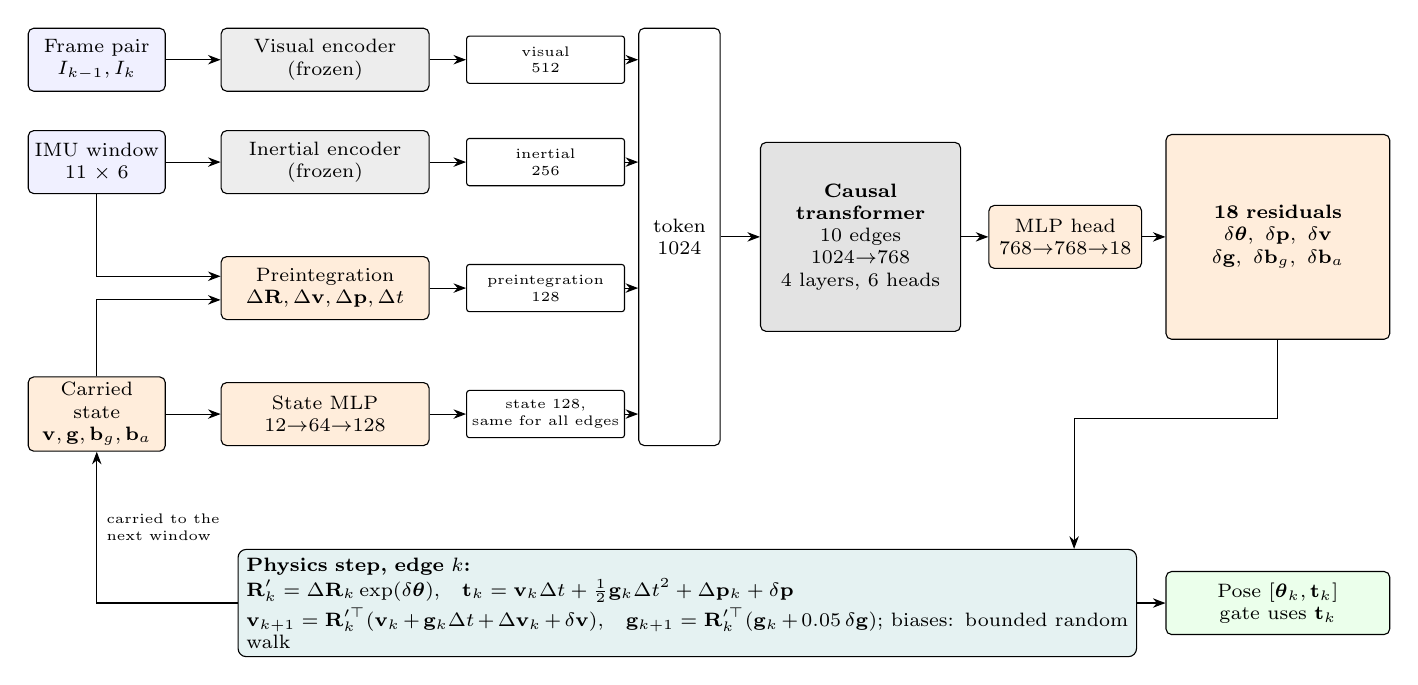
\begin{tikzpicture}[font=\scriptsize, >={Stealth[length=1.6mm]},
  blk/.style={draw, rounded corners=2pt, align=center, inner sep=2pt, minimum height=8mm, text width=#1},
  blk/.default=22mm,
  inp/.style={blk=16mm, fill=blue!6},
  enc/.style={blk=#1, fill=gray!14}, enc/.default=25mm,
  add/.style={blk=#1, fill=orange!14}, add/.default=25mm,
  tok/.style={draw, rounded corners=1pt, fill=white, align=center, inner sep=1.5pt, font=\tiny, text width=19mm, minimum height=6mm}]
\node[inp] (img) at (0.9,0) {Frame pair\\$I_{k-1},I_k$};
\node[inp] (imu) at (0.9,-1.3) {IMU window\\$11\times6$};
\node[blk=16mm, fill=orange!14] (st) at (0.9,-4.5) {Carried state\\$\mathbf v,\mathbf g,\mathbf b_g,\mathbf b_a$};
\node[enc] (venc) at (3.8,0) {Visual encoder\\(frozen)};
\node[enc] (ienc) at (3.8,-1.3) {Inertial encoder\\(frozen)};
\node[add] (pre) at (3.8,-2.9) {Preintegration\\$\Delta\mathbf R,\Delta\mathbf v,\Delta\mathbf p,\Delta t$};
\node[add] (smlp) at (3.8,-4.5) {State MLP\\$12{\to}64{\to}128$};
\node[tok] (tv) at (6.6,0) {visual\\512};
\node[tok] (ti) at (6.6,-1.3) {inertial\\256};
\node[tok] (tp) at (6.6,-2.9) {preintegration\\128};
\node[tok] (ts) at (6.6,-4.5) {state 128,\\same for all edges};
\node[draw, rounded corners=2pt, fill=white, align=center, minimum height=5.3cm, text width=8mm] (cat) at (8.3,-2.25) {token\\1024};
\node[blk=24mm, fill=gray!22, minimum height=24mm] (tf) at (10.6,-2.25) {\textbf{Causal transformer}\\10 edges\\$1024{\to}768$\\4 layers, 6 heads};
\node[add=18mm] (head) at (13.2,-2.25) {MLP head\\$768{\to}768{\to}18$};
\node[add=27mm, minimum height=26mm] (res) at (15.9,-2.25) {\textbf{18 residuals}\\$\delta\boldsymbol\theta,\ \delta\mathbf p,\ \delta\mathbf v$\\$\delta\mathbf g,\ \delta\mathbf b_g,\ \delta\mathbf b_a$};
\node[draw, rounded corners=3pt, fill=teal!10, inner sep=3pt, text width=112mm, align=left] (ph) at (8.4,-6.9) {\textbf{Physics step, edge $k$:}\\[1pt]
$\mathbf R'_k=\Delta\mathbf R_k\exp(\delta\boldsymbol\theta)$,\quad $\mathbf t_k=\mathbf v_k\Delta t+\tfrac12\mathbf g_k\Delta t^2+\Delta\mathbf p_k+\delta\mathbf p$\\[1pt]
$\mathbf v_{k+1}=\mathbf R_k'^{\top}(\mathbf v_k+\mathbf g_k\Delta t+\Delta\mathbf v_k+\delta\mathbf v)$,\quad $\mathbf g_{k+1}=\mathbf R_k'^{\top}(\mathbf g_k+0.05\,\delta\mathbf g)$;\ biases: bounded random walk};
\node[blk=27mm, fill=green!8] (out) at (15.9,-6.9) {Pose $[\boldsymbol\theta_k,\mathbf t_k]$\\gate uses $\mathbf t_k$};
\draw[->] (img) -- (venc); \draw[->] (imu) -- (ienc);
\draw[->] (imu.south) |- ([yshift=1.5mm]pre.west);
\draw[->] (st.north) |- ([yshift=-1.5mm]pre.west);
\draw[->] (st) -- (smlp);
\draw[->] (venc) -- (tv); \draw[->] (ienc) -- (ti); \draw[->] (pre) -- (tp); \draw[->] (smlp) -- (ts);
\foreach \t in {tv,ti,tp,ts} {\draw[->] (\t.east) -- (\t.east-|cat.west);}
\draw[->] (cat) -- (tf); \draw[->] (tf) -- (head); \draw[->] (head) -- (res);
\draw[->] (res.south) -- ++(0,-1.0) -| ([xshift=-8mm]ph.north east);
\draw[->] (ph.east) -- (out.west);
\draw[->] (ph.west) -| node[pos=0.75, right, font=\tiny, text width=17mm, align=left]{carried to the next window} (st.south);
\end{tikzpicture}
\caption{PI-VIFT. Orange: what it adds to VIFT. Besides the visual and inertial latents, each edge token carries a preintegration token and a state token. The head outputs 18 residual corrections; the physics step adds them to a kinematic prediction (rotation $\Delta\mathbf R_k$ from the gyroscope, translation from the carried velocity, gravity and the preintegrated acceleration), updates velocity, gravity and biases edge by edge, and carries the state to the next window. $\Delta\mathbf R_k,\Delta\mathbf v_k,\Delta\mathbf p_k$ come from preintegrating the IMU window with the current biases.}
\label{fig:pivift}
\end{figure*}

\subsection{Rotation from the gyroscope}
We integrate the raw gyroscope over the true image interval, $\Delta\mathbf{R}_k=\prod_i \exp([\bar{\boldsymbol{\omega}}_i-\mathbf{b}_g]_\times\,\Delta t_i)$, with the bias $\mathbf{b}_g$ taken from a static start where the sequence has one (EuRoC) and zero otherwise (KITTI, and the TUM-VI rooms, whose bias is below 0.002\,rad/s), and rotate it into the camera frame with the calibrated extrinsic (Fig.~\ref{fig:timing}). Rotation comes from the gyroscope, except inside KITTI OXTS outages longer than 50\,ms, where the network rotation is kept ($\le$0.01\% effect).

\subsection{Direction from two-view geometry}
With $\mathbf{R}_k$ known, each tracked corner pair (bearings $\mathbf{x}_A,\mathbf{x}_B$) gives one linear constraint $\mathbf{t}^\top\big((\mathbf{R}_k\mathbf{x}_B)\times\mathbf{x}_A\big)=0$, so two corners fix the direction. We track corners with forward--backward Lucas--Kanade, undistort them (radial--tangential or equidistant fisheye, limited to 60$^\circ$ off-axis), run two-point RANSAC with a 1\,px epipolar threshold, refit on the inliers by SVD and fix the sign by cheirality. The first-order uncertainty $\sigma_{\mathrm{geo}}$ follows from the singular values; below 2\,px of de-rotated parallax the direction is re-measured over 200 or 300\,ms. An edge has no geometric direction, and keeps the network's, when fewer than 15 corners are tracked, the median de-rotated parallax is below 0.5\,px, or RANSAC keeps fewer than 15 inliers or fewer than half of the matches; geometry is available on 85--96\% of the EuRoC edges and on 88--95\% of the edges of TUM-VI rooms 1--4.

\subsection{Length from the accelerometer}
Over a window of $W$ consecutive edges we solve a linear alignment \cite{Qin2017} for the initial velocity $\mathbf v_0$, gravity $\mathbf g$, accelerometer bias $\mathbf b_a$ (with a ridge prior) and the $W$ step lengths $\ell_k$, given gyro attitudes, preintegrated accelerations and the edge directions $\mathbf d_k$:
\begin{align}
\mathbf R_k\mathbf R_{bs}\,\mathbf d_k\,\ell_k &= \mathbf v_k\Delta t_k+\tfrac12\mathbf g\,\Delta t_k^2\nonumber\\
&\quad+\mathbf R_k(\boldsymbol\alpha_k-\mathbf J_{\alpha,k}\mathbf b_a)+(\mathbf R_{k+1}-\mathbf R_k)\mathbf p_{bs},\label{eq:align}\\
\mathbf v_k &= \mathbf v_0+\mathbf g\,T_k+\textstyle\sum_{j<k}\mathbf R_j(\boldsymbol\beta_j-\mathbf J_{\beta,j}\mathbf b_a),\nonumber
\end{align}
where $\boldsymbol\alpha_k,\boldsymbol\beta_k$ are the position and velocity increments preintegrated from the raw accelerometer over edge $k$, $\mathbf J$ their Jacobians with respect to the bias, $\mathbf R_k$ the gyro attitude, $\mathbf R_{bs}$ the camera-to-IMU rotation, $\mathbf p_{bs}$ the camera lever arm and $T_k$ the time since the window start. Each edge gives three equations, so $3W$ equations are linear in $9+W$ unknowns; a ridge row (weight 1) pulls $\mathbf b_a$ toward zero, and the \emph{alignment misfit} is the RMS of the residuals, in metres. Windows are disjoint; a KITTI window containing an OXTS gap longer than 50\,ms keeps the network length. $W$ is 500 edges on KITTI ($\approx$52\,s, chosen on training drives) and 20 on EuRoC and TUM-VI (2\,s). A window is used if it is observable: on KITTI if its design matrix has condition number below $10^4$, on EuRoC and TUM-VI if its gravity estimate lies within 0.5\,m/s$^2$ of 9.81; otherwise the network length is kept.

\subsection{The observability gate}
Rotation is the gyroscope's. For the direction, let $\sigma_g^2=\sigma_{\mathrm{geo}}^2+(A/p)^2$, where $p$ is the de-rotated parallax and $A=6.755^\circ$\,px a floor fitted on KITTI training drives. If $\angle(\dnet,\dgeo)\le 3\sqrt{\sigma_g^2+\sigma_{\mathrm{net}}^2}$, the two are fused with inverse-variance weights; otherwise $\dgeo$ replaces $\dnet$ when the angle exceeds $3\sigma_g$, and $\dnet$ is kept on the remaining edges. Each length window is solved with both $\dnet$ and the gated direction, keeping the solution with the smaller alignment misfit, so a few wrong directions cannot corrupt a window. In the pre-registered version (v3), $\sigma_{\mathrm{net}}=0.83^\circ$, the network's median direction error on held-out KITTI 08. Fig.~\ref{fig:gate} summarizes the decisions.

\begin{figure}[t]
\centering
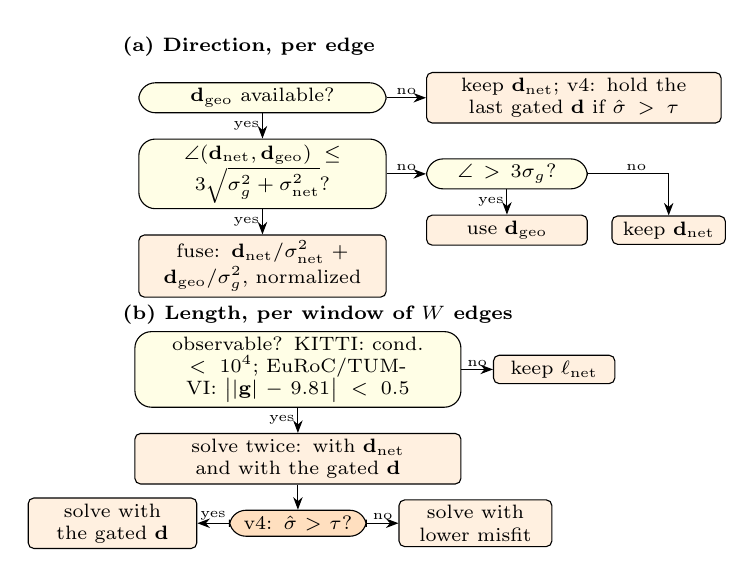
\begin{tikzpicture}[font=\scriptsize, >={Stealth[length=1.6mm]}, node distance=3.2mm,
  q/.style={draw, rounded corners=6pt, fill=yellow!10, align=center, inner sep=2pt, text width=#1},
  q/.default=30mm,
  a/.style={draw, rounded corners=2pt, fill=orange!12, align=center, inner sep=2pt, text width=#1},
  a/.default=19mm,
  v4/.style={draw, rounded corners=6pt, fill=orange!25, align=center, inner sep=2pt, text width=#1},
  v4/.default=19mm,
  yn/.style={font=\tiny, inner sep=1pt},
  ttl/.style={font=\scriptsize\bfseries, anchor=west}]
% (a) direction
\node[ttl] (ta) at (-1.9,0.35) {(a) Direction, per edge};
\node[q] (d1) at (0,-0.3) {$\dgeo$ available?};
\node[q, below=of d1] (d2) {$\angle(\dnet,\dgeo)\le 3\sqrt{\sigma_g^2+\sigma_{\mathrm{net}}^2}$?};
\node[a, below=of d2, text width=30mm] (fuse) {fuse: $\dnet/\sigma_{\mathrm{net}}^2+\dgeo/\sigma_g^2$, normalized};
\node[q, right=5mm of d2, text width=19mm] (d3) {$\angle > 3\sigma_g$?};
\node[a, below=of d3] (geo) {use $\dgeo$};
\node[a, right=3mm of geo, text width=13mm] (net1) {keep $\dnet$};
\node[a, right=5mm of d1, text width=36mm] (nogeo) {keep $\dnet$; v4: hold the last gated $\mathbf{d}$ if $\hat\sigma>\tau$};
\draw[->] (d1) -- node[yn, above]{no} (nogeo);
\draw[->] (d1) -- node[yn, left]{yes} (d2);
\draw[->] (d2) -- node[yn, left]{yes} (fuse);
\draw[->] (d2) -- node[yn, above]{no} (d3);
\draw[->] (d3) -- node[yn, left]{yes} (geo);
\draw[->] (d3.east) -| node[yn, pos=0.3, above]{no} (net1.north);
% (b) length
\node[ttl] (tb) at (-1.9,-3.05) {(b) Length, per window of $W$ edges};
\node[q, text width=40mm] (l1) at (0.45,-3.75) {observable? KITTI: cond.\ $<10^4$; EuRoC/TUM-VI: $\big||\mathbf{g}|-9.81\big|<0.5$};
\node[a, right=4mm of l1, text width=14mm] (lnet) {keep $\ell_{\mathrm{net}}$};
\node[a, below=of l1, text width=40mm] (solve) {solve twice: with $\dnet$ and with the gated $\mathbf{d}$};
\node[v4, below=of solve, text width=16mm] (t2) {v4: $\hat\sigma>\tau$?};
\node[a, left=4mm of t2, text width=20mm] (gsol) {solve with the gated $\mathbf{d}$};
\node[a, right=4mm of t2, text width=18mm] (mis) {solve with lower misfit};
\draw[->] (l1) -- node[yn, above]{no} (lnet);
\draw[->] (l1) -- node[yn, left]{yes} (solve);
\draw[->] (solve) -- (t2);
\draw[->] (t2) -- node[yn, above]{yes} (gsol);
\draw[->] (t2) -- node[yn, above]{no} (mis);
\end{tikzpicture}
\caption{Gate decisions. (a) Direction: fused where network and geometry agree within their combined uncertainty, geometry where they clearly disagree, network otherwise; without geometry, v4 holds the last gated direction once the network is distrusted. (b) Length: the accelerometer where its window is observable, the network elsewhere. Rotation always comes from the gyroscope. v3 uses a fixed $\sigma_{\mathrm{net}}=0.83^\circ$; v4 replaces it by the online $\hat\sigma$.}
\label{fig:gate}
\end{figure}

\textbf{Online trust (v4).} A fixed $\sigma_{\mathrm{net}}$ assumes the network is as good everywhere as on KITTI. v4 estimates it causally without ground truth: $\hat\sigma(k)$ is the median angle between $\dnet$ and $\dgeo$ over the last 100 \emph{confident} edges (geometry present, $p\ge5$\,px, $\sigma_g\le1^\circ$), with the 0.83$^\circ$ prior until 20 such edges exist. If $\hat\sigma>\tau=10^\circ$, edges without geometry hold the last gated direction and the length windows use only the gated direction. The confidence constants were fixed from first principles and $\tau$ was selected on held-out data (Sec.~\ref{sec:gate}).

\textbf{Runtime.} The measurement side costs 39--41\,ms per 100\,ms edge on one Apple M1 Pro core (512$\times$512 fisheye frames), 2.5$\times$ faster than real time; the network runs unchanged on the GPU.

\section{Experiments}

\subsection{Setup and protocol}
\textbf{Data.} KITTI odometry \cite{Geiger2012} (training 00, 01, 02, 04, 06, 09, plus 08 in one split; test 05, 07, 10); EuRoC \cite{Burri2016} (training MH\_01--04 and V2\_01, validation V1\_03, test MH\_05, V2\_02, V1\_01, V1\_02, with the ground-truth quaternion order corrected); TUM-VI \cite{Schubert2018} (training room1--4, test room5--6; 16-bit frames converted to 8 bits, as a naive conversion saturates every frame).
\textbf{Networks.} KITTI: VIFT retrained with our recipe (angle-weighted L1), 3 seeds per split, with mirror augmentation on the clean split. EuRoC: VIFT-style and PI-VIFT (Sec.~\ref{sec:learned}), 3 seeds each; the 4-sequence gate runs use PI-VIFT seed 123 and a single-seed PI-VIFT trained with a direction loss. TUM-VI: PI-VIFT fine-tuned from the EuRoC checkpoints, 3 seeds. Cross-model: VS-VIO \cite{Yang2022} with its released weights (trained with 08).
\textbf{Metrics and references.} KITTI $t_\mathrm{rel}$ and $r_\mathrm{rel}$ over 100--800\,m segments, against the OXTS ground truth and against SuMa lidar-SLAM poses \cite{Behley2018}, which do not use the IMU; EuRoC and TUM-VI SE(3) ATE on the 10\,Hz edge chain, next to the zero-motion floor.
\textbf{Protocol.} VIFT's released code trains on 08 although its paper excludes it, and selects checkpoints on the test drives. Our headline (\emph{clean}) protocol uses the paper's split and selects on held-out 08; the released-code split, with checkpoints selected on the test drives as in VIFT's code, is reported as secondary. Gate constants were fixed on training or held-out data and the success criterion was registered before a single test run: match or beat the better hand-designed pipeline within 0.05 $t_\mathrm{rel}$ (KITTI) or 0.1\,m (EuRoC, TUM-VI). One deviation: the registered text required both length checks of Sec.~\ref{sec:method} on every dataset, while the code that produced all results applies one per dataset.

\subsection{KITTI}

\begin{table}[t]
\caption{KITTI 05/07/10, $t_\mathrm{rel}$\,\% (mean $\pm$ sd over 3 seeds) / $r_\mathrm{rel}$. Clean: paper-text split, checkpoint selected on held-out 08. With 08: checkpoint selected on the test drives, as in VIFT's code. SuMa: lidar-SLAM reference independent of the IMU; against SuMa, $r_\mathrm{rel}$ is 0.32 for every row with gyro rotation.}
\label{tab:kitti}
\centering\small
\setlength{\tabcolsep}{3pt}
\resizebox{\columnwidth}{!}{\begin{tabular}{@{}lccc@{}}
\toprule
 & Clean, OXTS & Clean, SuMa & With 08, OXTS \\
\midrule
Network & 3.04$\pm$0.86 / 1.04 & 3.08 & 2.15$\pm$0.17 / 0.83 \\
+ gyro rotation & 2.10$\pm$0.04 / 0.18 & 2.20 & 1.61$\pm$0.07 / 0.18 \\
+ accel.\ length & 1.62$\pm$0.03 / 0.18 & 1.71 & 1.27$\pm$0.07 / 0.18 \\
\textbf{Gate (v3 = v4)} & \textbf{1.56$\pm$0.02} / 0.18 & \textbf{1.65} & \textbf{1.21$\pm$0.06} / 0.18 \\
\midrule
VIFT + RPMG \cite{Kurt2024} & \multicolumn{3}{l}{1.96 / 0.46 (no 08, selected on test)} \\
DB-VIO \cite{Wan2026} & \multicolumn{3}{l}{1.77 / 0.69 (split not confirmed)} \\
MixVIO \cite{Ma2026} & \multicolumn{3}{l}{1.69 (abstract)} \\
DAP-Pose, cam+IMU / +GNSS \cite{DAPPose} & \multicolumn{3}{l}{1.90 / 0.54; 1.31 / 0.46 (with 08)} \\
\bottomrule
\end{tabular}}
\end{table}

Table~\ref{tab:kitti} gives the main result. The gyroscope removes most of the error (3.04$\to$2.10\% clean, $r_\mathrm{rel}$ 1.04$\to$0.18; Fig.~\ref{fig:heading}), the accelerometer length most of the rest (1.62\%), and the gate, which measures the length and fuses the direction, reaches 1.56\% without test-set selection, against VIFT's 1.96\%. $r_\mathrm{rel}$ 0.18 is measured against OXTS, which shares the unit with the gyroscope; against SuMa it is 0.32, close to the 0.25 disagreement between the two references. Against SuMa the numbers rise by about 0.1 point (1.65\%), and a calibration that never touches OXTS ground truth (factory extrinsic, lag fitted against SuMa) gives 1.69\% for the hand-designed pipeline, so the gain is not an artifact of the IMU and the ground truth sharing a unit. On the released-code split the gate reaches 1.21\%. A network-free variant (gyro, fixed forward direction, accelerometer length, median length where unobservable) scores only 10.9\%: on a car the length is unobservable at stops and at constant speed, and there the network is needed. A caveat: on held-out 08 itself, gyro with network translation (0.86\%) beats both the accelerometer length (1.22\%) and the gate (1.20\%), most likely because the checkpoints were selected on 08.

\begin{figure}[t]
\centering
\includegraphics[width=\columnwidth]{figures/kitti_gyro_heading_error.png}
\caption{KITTI heading error vs distance on 05/07/10. The network heading wanders by 2--7$^\circ$; the gyroscope integrated over the true image intervals stays within about $\pm0.5^\circ$. The step on 05 near 1.13\,km lies in a 1.62\,s OXTS outage and appears in both, so it most likely comes from the ground truth.}
\label{fig:heading}
\end{figure}

\textbf{Cross-model check.} On VS-VIO with its authors' weights (learned visual policy), the same chain, with the gate frozen and run once, gives 2.35\% (network) $\to$ 1.81\% (gyro, $r_\mathrm{rel}$ 0.88$\to$0.17) $\to$ 1.38\% (accelerometer) $\to$ \textbf{1.27\%} (gate; 1.30\% against SuMa); with full vision 3.88$\to$1.59\%. The same chain, run once on the released weights of UL-VIO \cite{Park2024ULVIO} and of the two NASVIO variants \cite{Chen2023NASVIO} (flops, latency), gives 3.52$\to$\textbf{1.74}\%, 2.58$\to$\textbf{1.42}\% and 2.50$\to$\textbf{1.38}\% (OXTS; all three released models were trained with 08 in their split, so these are with-08 numbers). The diagnosis and the gate transfer to models we did not train.

\subsection{EuRoC}

\begin{table}[t]
\caption{EuRoC SE(3) ATE (m) on the 10\,Hz edge chain. Network-free and gate use the same sensors as the networks (cam0 + IMU).}
\label{tab:euroc}
\centering\small
\setlength{\tabcolsep}{3pt}
\resizebox{\columnwidth}{!}{\begin{tabular}{@{}lccccc@{}}
\toprule
& MH\_05 & V2\_02 & V1\_01 & V1\_02 & Mean \\
\midrule
Zero-motion floor & 6.84 & 2.12 & 1.85 & 1.77 & 3.15 \\
Learned (VIFT-style / PI-VIFT) & & & & & 4.02--4.98 \\
Network-free (measured only) & 1.00 & 0.24 & 2.47 & 0.35 & 1.02 \\
\textbf{Gate v3} (two models) & & & & & \textbf{0.94 / 0.99} \\
ORB-SLAM3 m.-inertial, ours, no LC & 0.060 & 0.047 & 0.037 & 0.024 & 0.042 \\
VINS-Mono \cite{Delmerico2018} (lit., Sim(3)) & 0.35 & 0.08 & 0.07 & 0.10 & 0.15 \\
\bottomrule
\end{tabular}}
\end{table}

On EuRoC (Table~\ref{tab:euroc}) the learned models sit above the zero-motion floor, while measuring every component without a network gives 1.02\,m. The gyro rotation is accurate to 0.008--0.021$^\circ$ per edge, the two-view direction to 1.1--2.0$^\circ$ and the accelerometer length to within 0.7--5\% (all except V1\_01, discussed below). Geometry is available on 85--96\% of the edges, and the gate, with the same configuration as on KITTI, reaches 0.94--0.99\,m. Classical VIO remains far ahead (ORB-SLAM3 run by us under the same protocol: 0.042\,m), so this result is a diagnosis of where learned VIO fails rather than a state of the art on EuRoC.

V1\_01 is above the floor for every learned and per-edge method. A per-edge check shows that V1\_01 never rests, so our static-start gyro bias fell back to zero while the true bias is about 0.076\,rad/s, a 0.46$^\circ$ rotation error per edge that biases every geometric direction. Estimating the bias from visual rotations instead (an offline estimate over the whole sequence, agreeing with the static bias within 0.003\,rad/s on the other sequences) brings V1\_01 to 0.92\,m without a network and 0.60\,m with the gate; since this was found on a test sequence we report it as a diagnostic and keep the original numbers.

\subsection{TUM-VI and the gate across datasets}
\label{sec:gate}

TUM-VI tests transfer to a handheld fisheye platform with motion-capture ground truth. Before any network output, each measurement was checked on the test rooms: gyro rotation 0.13--0.16$^\circ$ per edge, two-view direction 0.88--1.27$^\circ$ (fisheye), accelerometer length within 0.5\%. The network-free pipeline scores 0.80 / 0.13\,m on room5 / room6; on room5 it loses accuracy on steps shorter than 3\,cm. ORB-SLAM3 scores 0.028\,m.

\begin{table*}[t]
\caption{Gate v3 (pre-registered) and v4 (post-hoc, frozen, run once). KITTI: $t_\mathrm{rel}$\,\%; EuRoC, TUM-VI: ATE (m). Hand: best hand-designed pipeline for that dataset.}
\label{tab:gate}
\centering\small
\setlength{\tabcolsep}{8pt}
\begin{tabular}{@{}lcccc@{}}
\toprule
Data & Network & Hand & Gate v3 & Gate v4 \\
\midrule
KITTI clean (OXTS / SuMa) & 3.04 / 3.08 & 1.62 / 1.71 & 1.56 / 1.65 & 1.56 / 1.65 \\
KITTI with 08 & 2.15 & 1.27 & 1.21 & 1.21 \\
VS-VIO, policy / full vision & 2.35 / 3.88 & 1.38 / 1.69 & 1.27 / 1.59 & 1.27 / 1.59 \\
EuRoC, 4 seq.\ (2 models) & 5.47 / 6.60 & 1.02 & 0.94 / 0.99 & 0.95 / 0.98 \\
EuRoC, 2 seq.\ (5 models) & 3.98--5.30 & 0.62 & 0.66--0.90 & \textbf{0.57--0.59} \\
TUM-VI, seeds 123/42/7 & 5.0--8.8 & 0.47 & 0.56/0.92/0.59 & \textbf{0.47/0.47/0.47} \\
\bottomrule
\end{tabular}
\end{table*}

\textbf{Pre-registered result (v3).} Table~\ref{tab:gate}: without being told the dataset, the gate meets the criterion on KITTI and on EuRoC's 4-sequence means, and, run frozen on VS-VIO, beats the hand-designed chain there. On the two-sequence EuRoC runs, 3 of 5 miss the 0.1\,m tolerance. On TUM-VI it fails: 0.69\,m mean over three seeds against a limit of 0.57\,m, most of the loss on room5. Before v3, the pre-registered v1 and a post-hoc v2 had failed on KITTI, and those test results informed the diagnosis (Sec.~\ref{sec:history}); v3 itself was designed only on held-out 08.

\textbf{Why it fails, and v4.} $\sigma_{\mathrm{net}}=0.83^\circ$ describes the network on KITTI; on TUM-VI the network is tens of degrees off, so wherever it happens to agree with geometry the fusion over-weights it, and edges without geometry inherit its direction. v4 replaces $\sigma_{\mathrm{net}}$ by the online estimate of Sec.~\ref{sec:method}. It was designed only on held-out data: KITTI 08 and zero-shot predictions on TUM-VI room1--4. There $\hat\sigma$ recovers the KITTI value without ground truth (0.77--0.80$^\circ$ against 0.83$^\circ$) and flags the TUM-VI network as unreliable (25--74$^\circ$); the pre-declared rule selected $\tau=10^\circ$. Run once on every test set, v4 equals v3 where the network is good (KITTI, VS-VIO; $\hat\sigma\approx0.7^\circ$), fixes the two-sequence EuRoC runs (0.57--0.59 against 0.62 hand-designed) and reaches 0.47\,m on all TUM-VI seeds. There it equals the network-free pipeline: for a network that is tens of degrees off the gate stops doing harm, but the network adds nothing. Because v4 was motivated by a test failure and the KITTI and EuRoC test sequences had been used in earlier gate runs, we label it post-hoc.

\begin{figure}[t]
\centering
\includegraphics[width=\columnwidth]{figures/observability_measure_vs_learn.png}
\caption{When to measure and when to learn. (a) Network minus geometric direction error vs de-rotated parallax: on EuRoC measuring is better by 50--110$^\circ$, on KITTI the network is better by 0.3--0.5$^\circ$. (b) KITTI network minus accelerometer length error vs window condition number: below the gate threshold the accelerometer is better.}
\label{fig:observ}
\end{figure}

\subsection{Design history and constants}
\label{sec:history}

\begin{table}[t]
\caption{The four gate versions. KITTI: $t_\mathrm{rel}$\,\% on the with-08 split, OXTS; EuRoC: 4-sequence ATE (m, two models); TUM-VI: ATE (m, mean of three seeds). Hand-designed pipeline: 1.27, 1.02, 0.47.}
\label{tab:versions}
\centering\small
\setlength{\tabcolsep}{3pt}
\resizebox{\columnwidth}{!}{\begin{tabular}{@{}llccc@{}}
\toprule
 & Status & KITTI & EuRoC & TUM-VI \\
\midrule
v1 & pre-registered & 1.96 (fail) & 1.01 / 0.98 & not run \\
v2 & post-hoc & 1.99 (fail) & 1.00 / 0.96 & not run \\
v3 & one test run & \textbf{1.21} & 0.94 / 0.99 & 0.69 (fail) \\
v4 & post-hoc & \textbf{1.21} & 0.95 / 0.98 & \textbf{0.47} \\
\bottomrule
\end{tabular}}
\end{table}

\textbf{v1 and v2.} v1 (pre-registered) switched to geometry when $\angle(\dnet,\dgeo)>3\sqrt{\sigma_{\mathrm{geo}}^2+\mathrm{FLOOR}^2}$, with a constant FLOOR of 0.685$^\circ$, the median geometric error on KITTI training drives. It met the criterion on EuRoC (1.01 / 0.98\,m) but not on KITTI (with 08: 1.96 / 2.02\% against 1.27 / 1.32\% for the hand-designed pipeline; clean: 2.31 / 2.38\% against 1.62 / 1.71\%). It sent 10--19\% of the edges to geometry, the slow ones (median step 0.28--0.47\,m against 0.7--0.86\,m overall), where the geometric error is about 2.5$^\circ$ while $\sigma_{\mathrm{geo}}$ is about 0.13$^\circ$: a floor in degrees is the wrong error model, since the error grows as the parallax shrinks. v2 (post-hoc) models the floor in pixels, $A/p$ with $A=6.755^\circ$\,px; EuRoC was unchanged (1.00 / 0.96\,m) and KITTI still failed (1.99 / 2.05\%, geometry used on 7\% of the edges). v3 adds the inverse-variance fusion and the double length solve, was chosen among several candidates on held-out 08, and ran once on the test data.

\begin{table}[t]
\caption{Sensitivity to the KITTI condition-number bound ($W=500$). Training: share of edges that use the IMU length and the median relative error of those lengths. Test: $t_\mathrm{rel}$\,\%, mean of three seeds (with 08; no 08 with mirror augmentation).}
\label{tab:sens}
\centering\small
\setlength{\tabcolsep}{3pt}
\resizebox{\columnwidth}{!}{\begin{tabular}{@{}lcccc@{}}
\toprule
Bound & Edges using IMU & Length error & With 08 & No 08 \\
\midrule
$10^3$ & 2\% & 5.5\% & 1.61 & 1.96 \\
$\mathbf{10^4}$ (fixed) & 41\% & 1.2\% & 1.27 & 1.55 \\
$10^5$ & 55\% & 1.2\% & 1.27 & 1.55 \\
$10^6$ & 55\% & 1.2\% & 1.27 & 1.55 \\
\bottomrule
\end{tabular}}
\end{table}

\textbf{Constants.} The constants of the gate were fixed before the test results they affect: the factor $K=3$ (a conventional 3-sigma bound), the condition-number bound $10^4$, the gravity tolerance 0.5\,m/s$^2$ and the 50\,ms OXTS gap limit. Their derivation is not documented beyond that. Only the condition-number bound has a sensitivity analysis (Table~\ref{tab:sens}): the test result is identical from $10^4$ to $10^6$, and at $10^3$ almost every window falls back to the network. No sensitivity was run for $K$, the gap limit or the lag search range ($-80$ to $+80$\,ms; the fitted lags, $+60$ to $+65$\,ms, lie well inside it). Without the fallback, IMU-only lengths are fragile on the training drives (drive 04 is unobservable, drives 02 and 08 reach 2--9\% error), so the bound matters.

\section{Discussion and Limitations}

Fig.~\ref{fig:observ} summarizes the rule: the useful split between measured and learned components follows observability and differs between datasets, and the trust placed in the learned part should itself be measured, not assumed. A cheap oracle swap tells which component to fix first; on KITTI it avoids searching for better rotation losses.

\textbf{Limitations.} (i) KITTI's IMU and ground truth share the OXTS unit; SuMa and an OXTS-free calibration bound this effect (+0.1 point in $t_\mathrm{rel}$; $r_\mathrm{rel}$ 0.18$\to$0.32), and TUM-VI motion capture validates the estimators independently. (ii) v4 is post-hoc and needs confirmation on data unseen at every stage. (iii) The gate cannot beat its measurements: where neither geometry nor the network is reliable (TUM-VI room5's sub-3\,cm steps) nothing helps. (iv) The length check differs between datasets as implemented (condition number on KITTI, gravity norm on EuRoC/TUM-VI), and the pixel constants were not rescaled per camera. (v) Frame-to-frame estimation without windowed optimization remains about 25$\times$ behind ORB-SLAM3 run by us and 7$\times$ behind VINS-Mono as reported. (vi) The gyro bias needs a static start; an online visual estimate is the obvious next step. (vii) PI-VIFT's translation contains IMU-preintegrated displacement (Sec.~\ref{sec:learned}), so on EuRoC and TUM-VI the comparison between network length and accelerometer length is not between independent sources; we did not measure how much this matters. (viii) Several constants ($K$, the gap limit, the lag range) were fixed without a sensitivity analysis (Sec.~\ref{sec:history}).

\section{Conclusion}

Learned VIO fails in identifiable, dataset-dependent places, and an oracle swap finds them. Measuring what the sensors observe, keeping the learned network only for the rest, and measuring how far to trust it yields a single configuration that improves VIFT to 1.56\% on KITTI without test-set selection, brings EuRoC from 5.5--6.6\,m to below 1\,m, improves three released models we did not train, and, once its trust is estimated online (post-hoc), stops doing harm on a third dataset. Natural next steps are networks that predict only the unobservable components together with their uncertainty, and windowed optimization over the gated estimates.

\bibliographystyle{IEEEtran}
\bibliography{refs}

\end{document}
